\section{Simulative Evaluation of Hierarchical Caching Systems}\label{sec:hierarchical:simulative:simulative}

We develop an event-based simulation framework to evaluate the performance of content delivery networks.
The results derived from the simulative evaluation are used to validate the analytic models.
The simulation framework further allows considering complex system characteristics in the performance evaluation that are not covered by the analytic models, such as the transit costs charged on inter-domain links.

%A hierarchical content delivery network with bandwidth constraints has been evaluated by simulation in \cite{applegate2010optimal}.
%The impact of using edge resources with limited capacity for content delivery on QoE is evaluated by means of simulation in \cite{info3-inproceedings-2015-530}.
In the following we describe the simulation model and investigate the benefit of overlays networks in hierarchical caching systems.
We use the model for transit traffic, c.f. \refsec{sec:p2p:methodology}, to assess the potential to save costs produced by inter-domain traffic.

\subsection{Simulation Model}\label{sec:simeval}

The parameters considered in the content delivery simulation framework are
\begin{enumerate}
  \itemsep0em
  \item the resource distribution,
  \item the caching and content placement strategy,
  \item the resource selection strategy,
  \item the content demand,
  \item the AS-Topology.
\end{enumerate}
Other considered parameters that are not relevant for this monograph, are
\begin{enumerate}
  \itemsep0em
  \item the social network of users,
  \item the video bitrate and chunk-size distribution,
  \item and the application and QoE.
\end{enumerate}
In the following we briefly describe each of the parameter sets and provide models.

\subsubsection{Resource Distribution}
The resource distribution determines how video streaming sources are distributed among autonomous systems.
The number and size of autonomous systems is specified.
The size of an autonomous system is given by the number of end-users located in it.
In literature, the distribution of end-users on ASs is characterized as heterogeneous \cite{Hossfeld2011}.
We use a geometric distribution as a basic model for number of end-users in the ASs.
A more detailed model is developed using the Internet Census dataset, c.f. \refsec{sec:aslevel:census}.
Video streaming sources can be a) data centers of the content provider, b) edge caches of the content provider, c) caches hosted by the ISP, d) home router / NaDas, or e) end-user devices.
For each video streaming source the AS-location and its capacity is specified.
The capacity is given by the number of items that can be cached.
The size of the item catalogue is also specified in this parameter set.

The cache resources can have bandwidth constraints specified by the mean and the standard deviation of the upload bandwidth.
If the upload bandwidth of a cache is limited, the service time of an object is calculated according to the available bandwidth and the object size.
The service times of the objects served by a cache are updated if the upload bandwidth changes or if an object request arrives or is completed.
Requests are blocked by a cache if the available bandwidth is below a certain threshold, or if the cache is busy serving a request.

\subsubsection{Caching and Content Placement Strategy}
The caching and content placement strategy determines in which video streaming source which video item is placed and when.
The content placement strategy is defined by the caching strategies of the individual caches.
In a distributed approach each cache decides based on the information it has, which items to cache.
Thus, the availability of items in ASs might for example be increased.
If global knowledge of the item demand is assumed, optimized content placement strategies such as hot warm cold can be used.
Each caching strategy is further defined by its specific parameters according to \refsec{sec:hierarchical:background:strategies}.

\subsubsection{Resource Selection Strategy}
The resource selection strategy determines from which cache instance an item is streamed when requested.
The simplest resource selection just selects a random resource.
In hierarchical content delivery networks, resources in tier-1 are selected first, by default.
Other resource selection strategies that try to optimize different metrics were implemented.
E.g., local resource selection tries to save inter-domain traffic by prioritizing caches in the order: home router / NaDa in the same AS, ISP managed cache in the same AS, edge cache of content provider, data center of content provider.
%Further resource selection strategies that are not yet implemented could for example consider load balancing of the request based on the capacity of the caches.

\subsubsection{Social Network of Users}
The social network of users determines the friendship relationships between users. A basic model only defines the number of users in the system.
The number of friends of the user can be modeled by a power-law or geometric distribution.
A more detailed model specifies the friendship graph which consists of a node for each user and edges between users with friend relationships.
Friendship graphs have typical properties, such as a heavy-tailed in and out degree distribution.
In literature are different models for generating graphs with these properties.
A model used to generate social network graphs with varying size and density is the forest fire model \cite{leskovec2005graphs}.
We further specify the feed size as parameter that represents the news feed of social network platforms.
The news feed is updated in sharing events.
Videos which are on the news feed of a user are watched with high probability.
Categories are defined by specifying the probability that a user is interested in a particular category.

\subsubsection{Traffic and Popularity Model}
The content demand determines the request rates of the video items.
Different demand models are implemented in the simulation, that reach from basic models that only consider the popularity distribution of the items, to detailed models that consider temporal, spatial and social dynamics, c.f. \refsec{sec:hierarchical:background:traffic}.

The arrival process of video requests is specified by the inter-arrival time of video requests.
The request rate depends on the time of day and is generally lower at night.
The day is divided in short time slots, where the arrival rate does not change significantly, so that the arrival process can be assumed as quasi stationary.
In these time slots the arrival process is modeled as Poisson-process.
The parameter lambda of the arrival process depends on the popularity of the item and the time of day.
The probability of sharing a watched video is given by the sharing probability.

\subsubsection{Autonomous System Topology}
In order to estimate the amount of inter-domain traffic and transit costs produced, and AS topology with AS paths can be specified.
The AS paths connect the caches and data centers providing the content with the users consuming the content.
For that purpose the AS paths are inferred from AS relationships as in \refsec{sec:p2p:methodology}.
Assuming that the number of users is proportional to the number of IP addresses in an AS, we use the results of the Internet Census Dataset evaluation in \refsec{sec:aslevel:census}, to determine the distribution of users on ASs.

Finally, Simulation parameters are specified that define the random number seed, the simulation time and the parameter study.

\subsubsection{Performance metrics}

To assess the performance of content delivery networks several metrics are considered:

\begin{enumerate}
\item Cache hit rate: The ratio of requests to a cache that find the object in the cache (cache hit).
\item Cache serve rate: The ratio of requests to a cache that find the object in the cache and that are not blocked due to bandwidth constraints.
\item Cache contribution: The share of all requests that is served by a cache.
\item Inter-domain traffic: The share of requests by users in an AS that cannot be served by a cache in the same AS.
\end{enumerate}

\begin{figure}[bt]
  \centering
  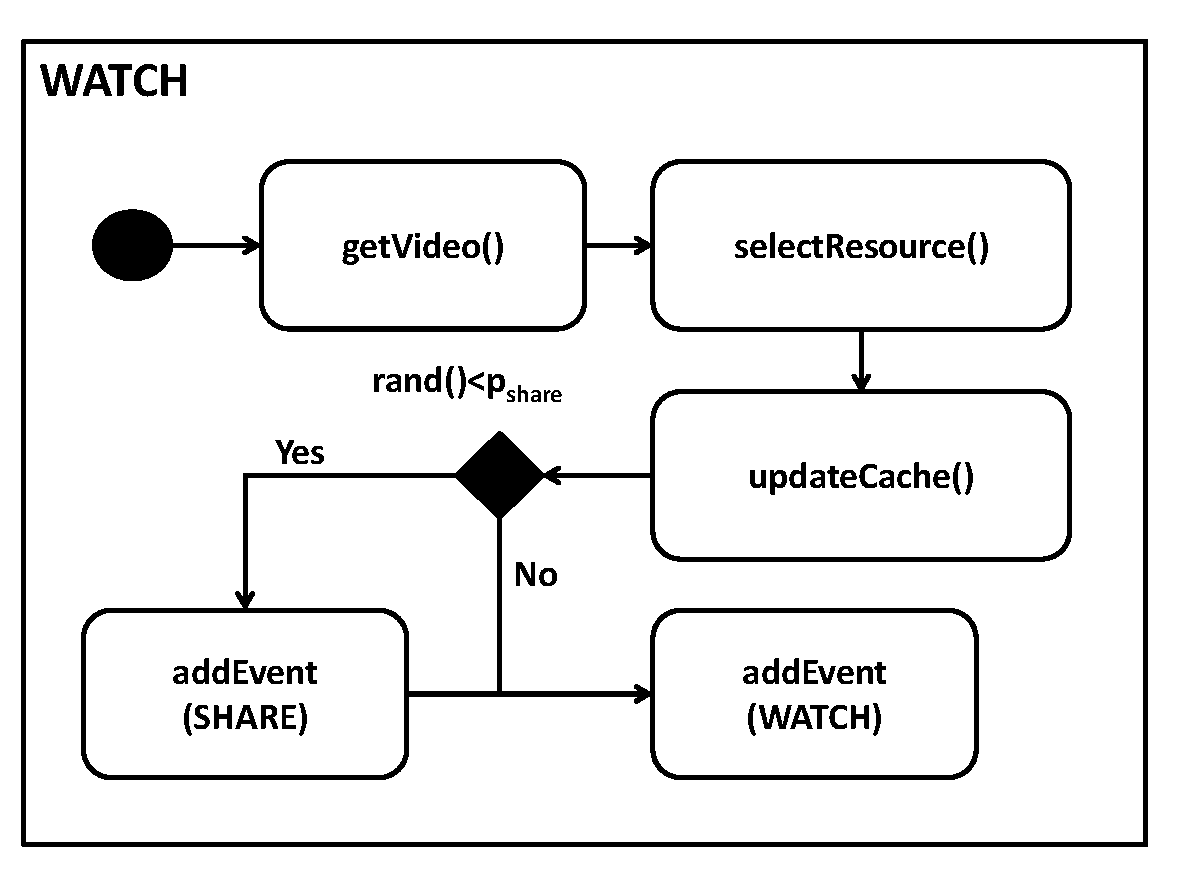
\includegraphics[width=0.6\textwidth]{hierarchical/simulative/figures/watch}
  \caption{Proccess diagram of a WATCH event.}
  \label{fig:WATCH}
\end{figure}

The content delivery simulation framework is implemented in MatLab.
The simulation is event-based including two major events.
First, the WATCH event, which is processed when a user watches or consumes a video item.
Second, the SHARE event, which simulates a sharing action of a user, where the video is posted on the news feeds in the social network.
\reffig{fig:WATCH} shows the process diagram of a WATCH event.
The process of a WATCH event starts by selecting a video according to the specified demand model.
A video identifier $v_\text{id}$ is returned.
In the next step a cache or data center is selected according to the resource selection strategy that holds the item with $v_\text{id}$.
The download of the item from the selected resource is recorded in the statistics.
The cache identifier $c_\text{id}$ is returned and the cached items are updated according to the caching strategy specified in the parameters.
The user then decides to share $v_\text{id}$ with probability $p_\text{share}$.
In this case a SHARE event is queued.
Finally, the next WATCH event is queued according to the traffic and popularity model.

A SHARE event puts a given $v_\text{id}$, or a random video according to the user's interest on top of the news feed of the user's friends.
The user's friends are determined by the social graph.
The simulation is initialized with a WATCH event for each user.

The simulation framework is open source and available on github\footnote{\url{https://github.com/pettitor/content_delivery}}.
